\chapter{Background and Related Work}
\label{chap:background}

This chapter introduces the theoretical foundation and specialized terminology in deep learning and computer vision that underpin this thesis. By defining core architectures, such as \acrfull{cnn}, \acrfull{rnn}, \acrfull{vit}, and \acrfull{s6}, the chapter establishes the theoretical basis for the experiments. Next, it explains the standard evaluation metric \acrfull{map}. The chapter then examines advanced video-analysis methodologies, including spatiotemporal convolutions, state-space models, and masked autoencoder frameworks. Finally, it reviews recent football-event-spotting research, such as COMEDIAN and VideoMAMBA, to identify specific limitations that motivate our proposed approach.

\section{Football Analytics}
\label{sec:football_analytics}

\subsection{Continuous Nature of Football}
Unlike sports with discrete plays, such as baseball or cricket, football is a continuous and dynamic domain. For example, a goalkeeper's pass during uninterrupted action generates numerous possible temporal sequences and starting conditions. This constant flow challenges event-based models. They identify individual occurrences and sequence-based models, which analyze ordered temporal inputs. Consequently, traditional discrete frameworks must be extended to preserve contextual data across continuous match sequences. 

\subsection{Data Sources and Key Metrics}
Football analytics rely on two primary data streams:

\begin{figure}
    \centering
    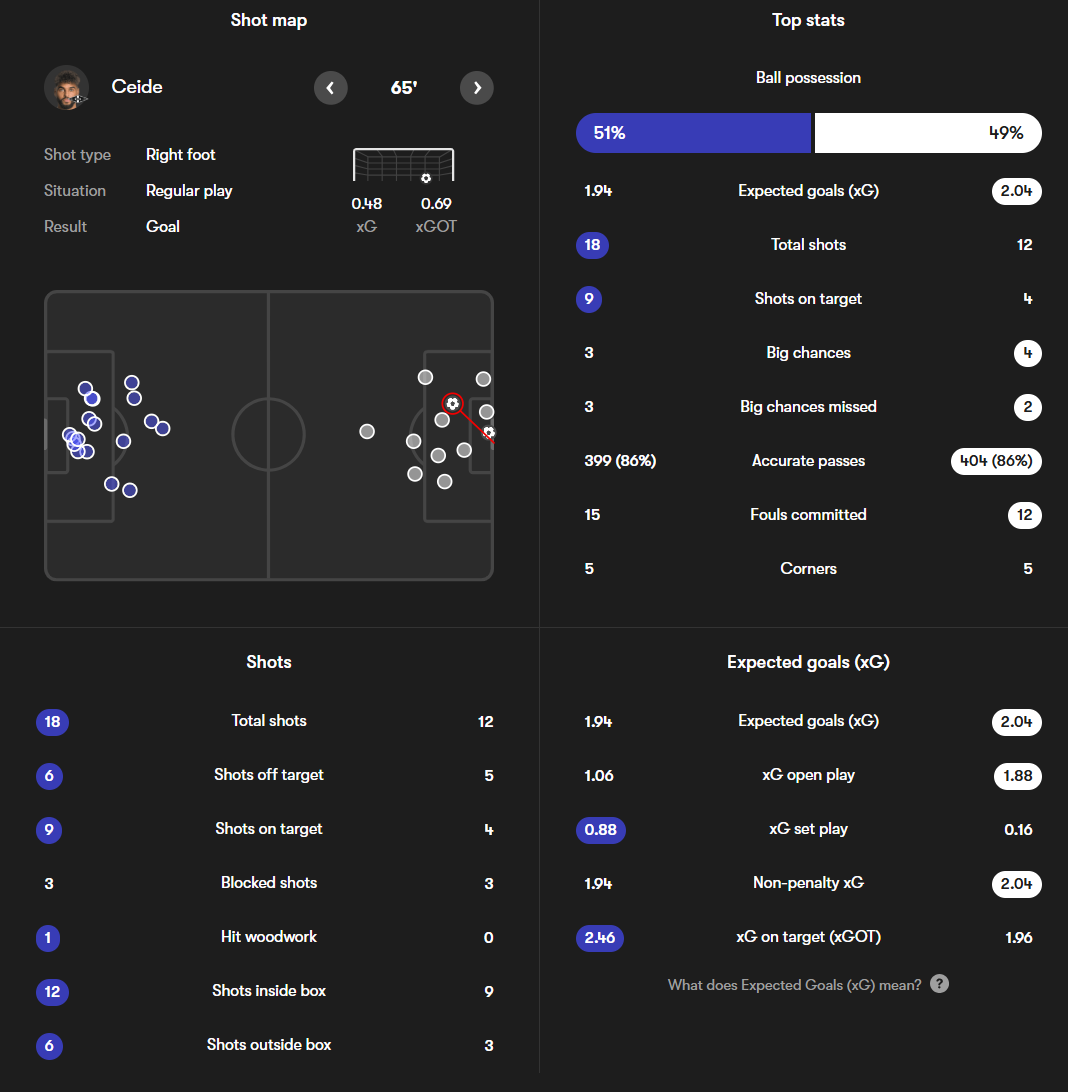
\includegraphics[width=0.66\linewidth]{figures/fotmob_rbk.png}
    \caption{Commercially available stats from a football game. Retrieved from FotMob\cite{fotmob_game}.}
    \label{fig:fotmob_stats}
\end{figure}

\begin{itemize}
    \item Event data: manually or commercially annotated discrete occurrences (shots, corners).
    \begin{itemize}
        \item \acrfull{xg}: estimates shot quality using spatial and contextual features with XGBoost trained on large historic datasets \cite{mead_xg_2023}.
        \item Set pieces (corners, free kicks): naturally bounded events suitable for end-to-end predictive models.
        \item \autoref{fig:fotmob_stats} shows a selection of commercially available statistics. 
    \end{itemize}
    \item Tracking data: high-frequency player trajectories from GPS vests or manual optical systems.
    \begin{itemize}
        \item Physical metrics: distance covered, top speed, accelerations for workload monitoring and injury risk assessment \cite{hennessy_gps_tracker_2018}.
    \end{itemize}
\end{itemize}

\textcite{wang_tactic_ai_2024} applies deep graph neural networks to corners, a discrete sub-event of play. They deliver strong predictive and generalizable performance and have helped Liverpool FC succeed. 

\section{Datasets}
\label{sec:datasets}

\textcite{survey_of_survey} presents comprehensive tables of sports action datasets. \textcite{seweryn_survey_2023} detail football-specific collections.

\subsection{SoccerNet}

\textcite{deliege_soccernet-v2_dataset_2021} introduces SoccerNet-V2, offering 500 match recordings annotated with 17 football events.

In 2024, \textcite{deliege_soccernet-v2_dataset_2021} released seven new games annotated with 12 ball events and team annotations. There are approximately six times as many events in these seven videos as in the original 500. 

\subsection{UCF101}
UCF101 \cite{dataset:UCF101} comprises 13,320 YouTube clips spanning 101 human action categories. It serves as a standard benchmark for trimmed action recognition.

\subsection{THUMOS}
THUMOS \cite{dataset:thumos} includes over 13,000 temporally annotated instances from 20 action classes. It evaluates detection in untrimmed videos.

\subsection{HACS}
HACS \cite{dataset:hacs} comprises 1.55 million short clips across 200 action classes. It provides both trimmed classification clips and untrimmed temporal segments.

\subsection{ActivityNet}
The FineAction dataset \cite{dataset:fineaction} comprises 103,000 temporal instances across 106 fine-grained action categories, annotated in 17,000 untrimmed videos. It features dense, co-occurring action annotations and rich class diversity. FineAction offers a new benchmark for detailed temporal action localization.


\subsection{Kinetics}
Kinetics-400/600/700 \cite{dataset:kinetics} provides hundreds of thousands of 10-second clips, each labeled with one of 400-700 action classes. The clips are from YouTube.

\subsection{FineAction}
FineAction \cite{dataset:fineaction} provides 10,000+ short clips of soccer actions annotated at the frame level with player bounding boxes. It enables fine-grained event spotting and player-centric analysis.



% \section{Datasets}
% \label{sec:datasets}

% \textcite
% Several large-scale video datasets have been developed to advance action recognition research. \textcite{survey_of_survey} provides comprehensive overviews of available sports-related action datasets (see their Tables 4 & 5), while Seweryn et al.~\cite{seweryn_survey_2023} focus specifically on football-centric collections. Below, we summarize the main datasets examined in this thesis, ordered by their relevance and scale.


% \subsection{SoccerNet-V2}
% \label{ssec:soccernet}

% The SoccerNet-V2 dataset \cite{deliege_soccernet-v2_dataset_2021} contains video recordings of 7 professional football matches with fine-grained annotations for 12 action classes. It provides:
% \begin{itemize}
%     \item 7 full matches (90 min each) at 25 fps.
%     \item Timestamped action labels for spotting tasks.
%     \item Team annotations for each event.
%     \item Publicly accessible via HuggingFace\footnote{\url{https://huggingface.co/datasets/SoccerNet/SN-BAS-2025}}.
%     \item The twelve football event classes:
%         \begin{center}
%             \begin{tabular}{llll}
%                 Pass & Drive & Header & High Pass \\
%                 Out & Cross & Throw In & Shot \\
%                 Ball Player Block & Player Successful Tackle & Free Kick & Goal
%             \end{tabular}
%         \end{center}
%     \item An action approximately every 3 seconds. 
% \end{itemize}

% The original SoccerNet dataset records 500 games with 17 action classes. 


% \subsection{THUMOS'14}
% \label{ssec:thumos}

% The THUMOS'14 dataset \cite{dataset:thumos} comprises:
% \begin{itemize}
%     \item 20 action classes in sports and daily activities.
%     \item 213 untrimmed videos for temporal detection.
%     \item Predefined train/val/test splits for benchmarking.
% \end{itemize}

\section{Deep Learning} 
\label{sec:deep_learning}

Deep learning comprises multilayer neural networks that automatically learn hierarchical data representations. By contrast, classical methods rely on handcrafted features; deep architectures, on the other hand, discover interesting patterns from raw inputs. They stack linear transformations and non-linear activations to extract meaningful features at each layer \cite{lecun_deep_learning_2015}. 
Early layers capture low-level primitives, while deeper layers combine these primitives into high-level concepts. Model training uses backpropagation to compute loss gradients with regard to millions of parameters. 

\subsection{Forward pass}
For a network with two hidden layers, the forward pass is:
\begin{align}
z^{(1)} &= W^{(1)} x + b^{(1)}, & y^{(1)} &= f\bigl(z^{(1)}\bigr), \\
z^{(2)} &= W^{(2)} y^{(1)} + b^{(2)}, & y^{(2)} &= f\bigl(z^{(2)}\bigr), \\
z^{(3)} &= W^{(3)} y^{(2)} + b^{(3)}, & \hat{y} &= g\bigl(z^{(3)}\bigr).
\end{align}
Here, \(x\in\mathbb{R}^d\) is the input, \(W^{(l)},b^{(l)}\) are weights and biases at layer \(l\), \(f(.)\) is an activation function (e.g. ReLU). Figure~\ref{fig:forward_pass} illustrates these computations. In the case of a classification task, \(g\) is the output activation (e.g., softmax), and \(\hat{y}\) is the predicted class.

\begin{figure}[ht]
    \centering 
    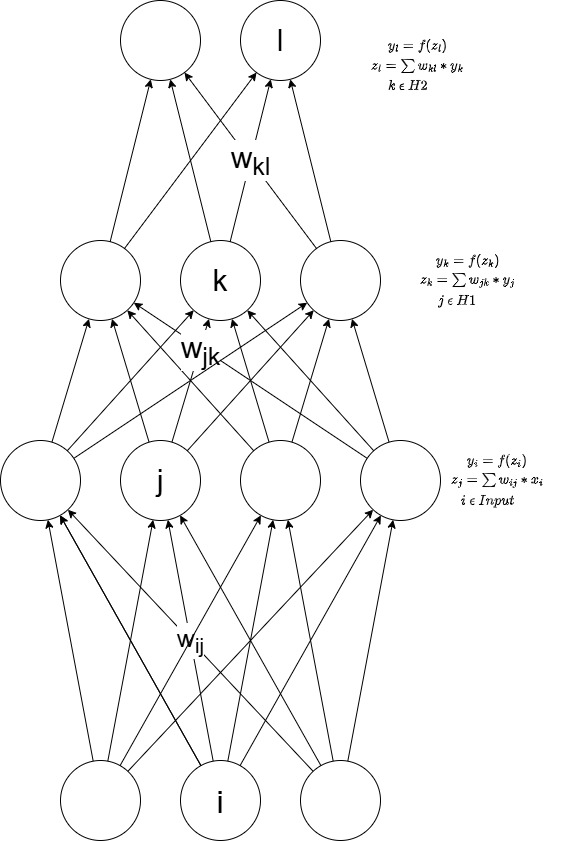
\includegraphics[width=0.6\linewidth]{figures/neural_net.jpg}
    \caption{Feedforward pass of a neural network with two hidden layers.} 
    \label{fig:forward_pass}
\end{figure}

\subsection{Backward pass}
Training minimizes a loss \(E(\hat y, y^\star)\), using, e.g., cross-entropy. Gradients are computed via the chain rule:
\begin{align}
\delta^{(3)} &= \frac{\partial E}{\partial z^{(3)}}
= \frac{\partial E}{\partial \hat y}\odot g'\bigl(z^{(3)}\bigr),\\
\delta^{(l)} &= \frac{\partial E}{\partial z^{(l)}}
= \bigl(W^{(l+1)\top}\delta^{(l+1)}\bigr)\odot f'\bigl(z^{(l)}\bigr),
\quad l=2,1.
\end{align}
Weight and bias gradients follow:
\begin{align}
\nabla_{W^{(l)}}E &= \delta^{(l)}\,y^{(l-1)\top}, &
\nabla_{b^{(l)}}E &= \delta^{(l)},
\end{align}
with \(y^{(0)}\equiv x\). Figure~\ref{fig:backward_pass} shows the backpropagation flow.

\begin{figure}[ht]
    \centering
    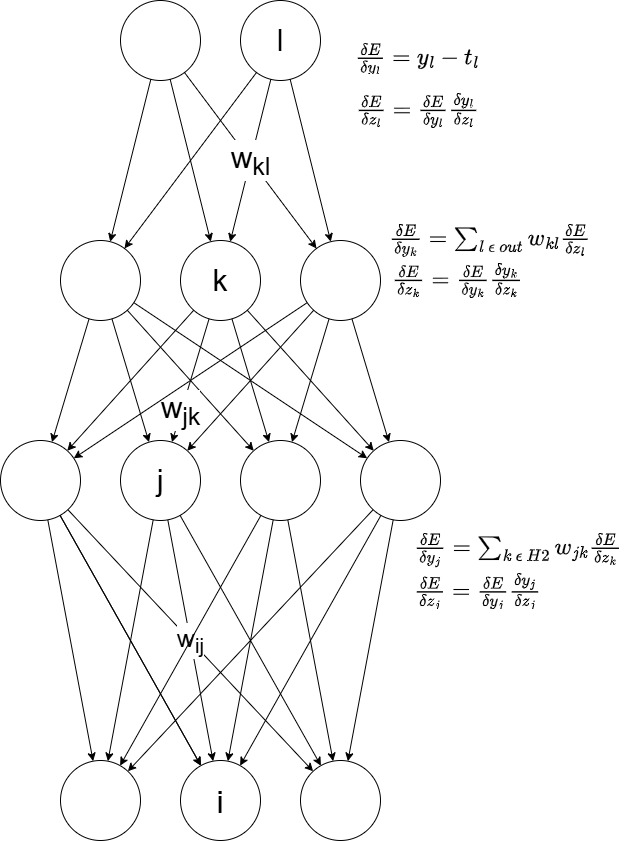
\includegraphics[width=0.6\linewidth]{figures/neural_net_back_prop.jpg}
    \caption{The equations that compute the backward pass.}
    \label{fig:backward_pass}
\end{figure}

\subsection{Optimization}
Parameters are updated using stochastic gradient descent (SGD) or adaptive variants, such as Adam and RMSprop. For learning rate \(\eta\),
\[
W^{(l)} \leftarrow W^{(l)} - \eta\,\nabla_{W^{(l)}}E,
\quad
b^{(l)} \leftarrow b^{(l)} - \eta\,\nabla_{b^{(l)}}E.
\]
Regularization techniques such as weight decay, dropout, and batch normalization further improve generalization and training stability \cite{ioffe_batch_2015}.

\subsection{Convolutions}

Convolutions learn small filters that slide over the input to detect local features in both space and time. Each filter is a small tensor of weights that computes a weighted sum plus a bias at every position. Convolutions capture patterns such as edges, textures, and motion by sharing the same weights across all locations.  

In the most basic scenario, when there is a layer with input dimensions of \( (N, C_{in}, H, W)\) and output dimensions of \( (N, C_{out}, H_{out}, W_{out})\), the output can be accurately described as follows:

\[out(N_i, C_{out_j}=bias(C_{out_j})+\sum_{k=0}^{C_{in}-1}weight(C_{out_j},k)\star input(N_i,k)\]

The symbol \(\star\) represents this expression's valid 2D cross-correlation operation. Here, \textit{\textbf{N}} refers to the batch size, \textit{\textbf{C}} indicates the number of channels, \textit{\textbf{H}} represents the height of the input planes measured in pixels, and \textit{\textbf{W}} denotes the width measured in pixels\cite{pytorch_conv2d}. 

Key components:
\begin{itemize}
    \item \textbf{Stride}, \textbf{padding}, and \textbf{dilation} control the receptive field and output resolution.
    \item \textbf{Pooling} (max or average) reduces spatial dimensions and enforces translational invariance.
    \item \textbf{Batch normalization} stabilizes learning by normalizing activations per mini-batch.
    \item Non-linear activations (ReLU, Leaky-ReLU, etc.). 
\end{itemize}

\begin{figure}
    \centering
    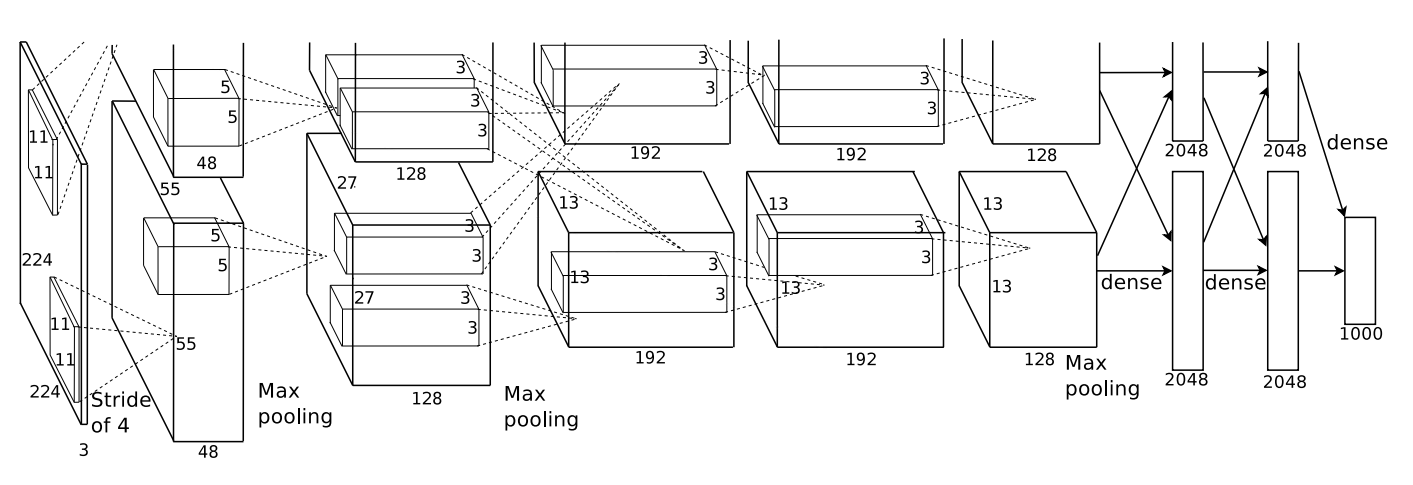
\includegraphics[width=1\linewidth]{figures/alexnet.png}
    \caption{An illustration of the architecture of AlexNet. One GPU runs the layer parts at the top of the figure, while the other runs the layer parts at the bottom. The figure and caption are Figure 2 in the released paper by \textcite{krizhevsky_alexnet}.}
    \label{fig:alexnet}
\end{figure}

Stacking multiple convolution-activation-pooling blocks builds hierarchical feature representations, from edges and textures in early layers to object parts in deeper layers \cite{lecun_deep_learning_2015}. \autoref{fig:alexnet} shows how \textcite{krizhevsky_alexnet} designed AlexNet in 2012 with alternating convolution and pooling layers. Residual connections \cite{he_deep_residual_2015} further ease training in very deep networks by learning residual mappings. \autoref{fig:res_connection} shows an example of a residual block. Architectures such as Inception \cite{szegedy_going_2014}, MobileNet (depthwise separable convolution) \cite{howard_mobilenets_2017}, and EfficientNet (compound scaling) \cite{tan_efficientnet_2020} optimize the trade-off between accuracy and efficiency in image tasks. 

\begin{figure}
    \centering
    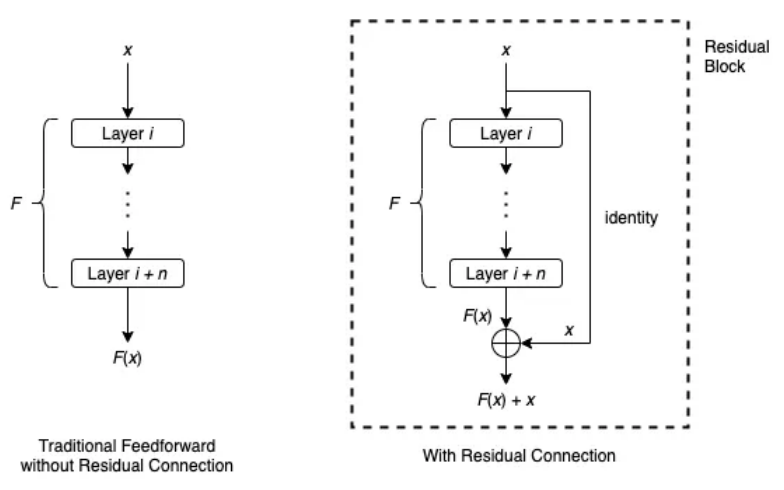
\includegraphics[width=0.5\linewidth]{figures/res_connection.png} 
    \caption{Residual block. Created by \textcite{wong_what_is_residual_2022}.}
    \label{fig:res_connection}
\end{figure}

In the video domain, spatiotemporal convolutions extend the same principles over time. Early 3D \acrshort{cnn}s \cite{tran_learning_2015} apply cubic kernels to capture motion but suffer high computational costs. The (2+1)D decomposition \cite{tran_2_plus_1_convolution} splits 3D kernels into separate spatial and temporal convolutions, improving the optimization. The \acrfull{i3d} \cite{carreira_2017_i3d_quo_vadis} "inflates" pre-trained 2D filters into the time dimension. \acrshort{i3d} creates a balance between efficiency and representation.

Further advances address long-range temporal modeling:
\begin{itemize}
    \item SlowFast networks \cite{feichtenhofer_slowfast_2019} use a dual-pathway: a \emph{Slow} branch at low frame rate for semantics and a \emph{Fast} branch at high frame rate for motion.  
    \item Temporal Shift Module (TSM) \cite{lin_temporal_shift_2019} achieves temporal modeling by shifting feature channels across frames with zero extra parameters.  
    \item X3D \cite{feichtenhofer_x3d_2020} systematically expands 2D image models into efficient, scalable 3D architectures by progressive width, depth and resolution scaling.
\end{itemize}

Despite their locality bias, \acrshort{cnn}-based video models remain foundational building blocks in modern action recognition frameworks. They are often combined with attention mechanisms to capture global spatiotemporal dependencies \cite{fu_look_2017}.


\subsubsection{\acrfull{gcn}}

\acrfull{gcn} is a subsection of Graph Neural Networks (GNNs), which accomplish link prediction, graph classification, and graph generation. \acrshort{gcn}s learns node embeddings. Each node has an identity, a vector, and is connected to other nodes. The idea is to aggregate information from its neighbours \cite{kipf_gcn_2017}.

\subsection{Recurrent Neural Nets}

\acrfull{rnn} are deep learning models designed to handle sequential data. 
\acrshort{rnn}s maintain a memory of previous inputs through feedback loops. It allows for information to persist across multiple time steps, unlike, for example, \acrshort{cnn}s and simple neural nets. The persistence of information makes \acrshort{rnn}s useful for tasks requiring temporal dependencies, such as natural language processing, speech recognition, and time-series forecasting\cite{ibm_rnn_2025}. In the context of \acrfull{cv}, \acrshort{rnn}s are applied to various applications, such as image captioning and video analysis. 

Standard \acrshort{rnn}s suffer from the vanishing gradient problem. The issue arises from the repeated multiplication of small gradient values during backpropagation through time. These small values result in diminishing updates in the early layers. \acrfull{lstm} is one solution to this problem \cite{bhogal_human_2023, kumar_human_2023, mahaseni_spotting_2021}.The other widespread solution is the \acrfull{gru} \cite{giveki_human_2024,li_oarnet_2024,yu_i3d_2023}. 

\subsubsection{\acrfull{lstm}}
\acrlong{lstm} introduce memory cells. The cells have input, forget, and output gates. \acrshort{lstm}s come with increased efficiency and increased complexity. On small datasets, \acrshort{lstm}s are prone to overfitting. 

\subsubsection{\acrfull{gru}}
\acrlong{gru}s use a reset gate and an update gate to maintain or discard information\cite{cho_gru_2014}. It has fewer parameters than an \acrshort{lstm}, which makes it more computationally efficient while addressing the vanishing gradient problem. \acrshort{gru}s are particularly attractive in scenarios with limited resources. 

\acrshort{rnn}-based architectures are used in video analysis models to capture temporal dependencies, like \textcite{bhogal_human_2023}. Although a historically popular resource for sequential data processing, transformer models have led to a decline in their usage. However, they remain relevant in contexts where step-by-step recurrence and memory provide distinct advantages \cite{ibm_rnn_2025}.

\subsubsection{Bi-Directional Layers}
\label{ssec:bi_directional_layers}

Bi-directional recurrent layers combine two parallel LSTM networks to capture past and future context in a sequence \cite{radhakrishnan_bi_lstm_2023, bhogal_human_2023}. One LSTM processes the input in its original order (forward pass), while the other processes it in reverse (backward pass). At each time step \(t\), the hidden states from both directions are concatenated to form a richer representation of the data:

\[
h_t = \bigl[\,\overrightarrow{h}_t;\,\overleftarrow{h}_t\bigr].
\]

In football analytics, this approach is helpful because events (e.g., \ goals, passes) often depend on both preceding and succeeding actions on the field. By integrating information from before and after a given frame, bi-directional layers can improve the accuracy of sequence predictions. The main trade-off is that they require roughly twice the number of parameters and incur longer training and inference times than unidirectional models.




\subsection{\acrfull{vit}}
\label{ssec:vision_transformers}

\acrlong{vit} adapt the transformer architecture \cite{vaswani_attention_2017} \change{Does transformers by themselves deserve a section?} to images by splitting each image into $P\times P$ patches, projecting them to $D$-dimensional embeddings, and adding positional encodings \cite{dosovitskiy_image_transformer_2021}. Given an image of size $H\times W$, one obtains
\[
\mathbf{x}_0 = [x_{\text{cls}};\,z_1,\dots,z_N] + E_{\text{pos}},
\]
$x_{\text{cls}}$ is a learnable classification token, and $E_{\text{pos}}\in\mathbb{R}^{(N+1)\times D}$ are positional embeddings, where $N=(H/P)\,(W/P)$,. The sequence is processed by $L$ identical blocks of multi-head self-attention (MSA) and feedforward networks (FFN)\cite{dosovitskiy_image_transformer_2021}:
\begin{align*}
y^l &= \mathrm{MSA}\bigl(\mathrm{LN}(x^{l-1})\bigr) + x^{l-1},\\
x^l &= \mathrm{FFN}\bigl(\mathrm{LN}(y^l)\bigr) + y^l,\quad l=1,\dots,L.
\end{align*}

TimeSformer \cite{bertasius_timesformer_2021} extends ViT to video by factorizing self-attention into separate spatial and temporal modules. It reduces complexity from $\mathcal{O}\bigl((TN)^2\bigr)$ to $\mathcal{O}(T^2N + N^2T)$. Formally, with tokens $z_{t,n}$ for frame $t$ and patch $n$,
\[
\mathrm{Attn}(Z)
= \mathrm{Softmax}\!\bigl(Q_sK_s^\top/\sqrt{D}\bigr)V_s
+ \mathrm{Softmax}\!\bigl(Q_tK_t^\top/\sqrt{D}\bigr)V_t.
\]

VViT \cite{arnab_vvit_2021} further improves video classification by combining factorized attention with multi-scale patch embeddings, achieving state-of-the-art results on multiple benchmarks.


Limitations of vision transformers include:
\begin{itemize}

    \item High data requirements—performance degrades on small or specialized datasets.  
    \item Computational cost—quadratic scaling with sequence length impacts memory and runtime.  
    \item Model complexity—large parameter counts increase overfitting risk \cite{lee_enhancing_mamba_s6_2024}.
\end{itemize}


\subsubsection{META \acrlong{sam}}
\label{ssec:meta_sam2}
\unsure{Move to the back of the chapter, or reference this part in the back of the chapter?}
The \acrfull{sam} was first introduced by \textcite{kirillov_segment_2023} in 2023 as a promptable, foundation segmentation model. Its core design splits the task into three components:
\begin{itemize}
    \item \textbf{Image Encoder:} A vision transformer (ViT) pre-trained on masked autoencoding produces dense feature maps for any input image.
    \item \textbf{Prompt Encoder:} A lightweight module that maps interactive prompts (points, bounding boxes, or free-form masks) into positional embeddings.
    \item \textbf{Mask Decoder:} A small transformer that fuses image and prompt embeddings to output segmentation masks at multiple scales.
\end{itemize}
SAM was trained on the enormous SA-1B dataset (over 11 M images and 1.1 B masks) in a semi-automated pipeline, yielding strong zero-shot performance across diverse domains without finetuning.

Building on this success, Ravi et al.\ \cite{ravi_sam_nodate} proposed \emph{SAM-2} (sometimes called Video \acrshort{sam}), which extends \acrshort{sam} to sequential video data via a \emph{memory-augmented attention} mechanism:
\begin{itemize}
    \item \textbf{Frame-wise Encoding:} Each video frame is encoded by the same ViT backbone used in image \acrshort{sam}.
    \item \textbf{Memory Attention:} A cross-frame attention layer that retains a compact set of "memory tokens" summarizing past masks, enabling consistent tracking of object masks over time.
    \item \textbf{Interactive Prompts in Video:} Mouse clicks and bounding-box prompts can be applied on any frame and propagated forward or backward via the memory bank.
\end{itemize}
The authors also released SA-V, a large video-segmentation dataset with millions of frame-mask pairs. Results on this dataset demonstrate that \acrshort{sam} achieves near real-time inference (15-30 fps) and high temporal consistency on common benchmarks. \autoref{fig:sa-v} shows the masklets in the dataset. 
\begin{figure}
    \centering
    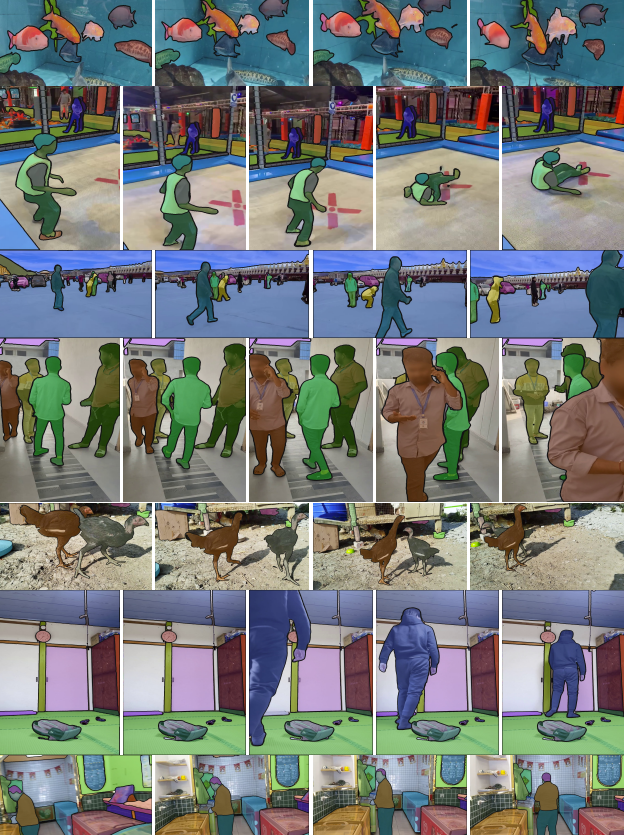
\includegraphics[width=0.5\linewidth]{figures/sam_2.png}
    \caption{Examples from the SA-V dataset. Figure 4 in the \acrshort{sam} paper\cite{ravi_sam_nodate}.}
    \label{fig:sa-v}
\end{figure}

Together, the original \acrshort{sam} and its video-centric successor exemplify a new paradigm in segmentation: a single, promptable transformer that can be deployed off-the-shelf, adapted to novel objects or domains with minimal human guidance, and extended from static images to dynamic scenes. 

\improvement{To increase readability, this section needs more figures, not only here}
\subsection{State-Space Models}
\label{ssec:state_space_models}
% \acrfull{ssm} offers a continuous-time representation of sequential data via a latent state \(h(t)\in\mathbb{R}^N\):
% \begin{align}
%     \frac{\mathrm{d}h(t)}{\mathrm{d}t} &= A\,h(t) + B\,x(t),  \label{eq:ssm_continuous1}\\
%     y(t) &= C\,h(t),                                    \label{eq:ssm_continuous2}
% \end{align}
% where \(x(t)\in\mathbb{R}^d\) is the input, \(y(t)\in\mathbb{R}^m\) the output, and \(A\in\mathbb{R}^{N\times N}, B\in\mathbb{R}^{N\times d}, C\in\mathbb{R}^{m\times N}\) are learned parameters.  Discretizing these equations with step size \(\Delta\) yields
% \begin{align}
%     \bar A &= \exp(\Delta\,A), 
%     & 
%     \bar B &= \bigl(\exp(\Delta\,A)-I\bigr)A^{-1}B,\\
%     h_k &= \bar A\,h_{k-1} + \bar B\,x_k, 
%     &
%     y_k &= C\,h_k,
%     \quad k=1,2,\dots
% \end{align}
% \unsure{Do I have to reference equations in the same way figures must be referenced in a text}
% VideoMamba \cite{li_videomamba_2024} builds on this framework with a \emph{Selective Scan} (\acrshort{s6}) core.  Its parameters \((\Delta, A,B,C)\) control:
% \begin{itemize}
%     \item \(\Delta\): temporal resolution of the recurrence,
%     \item \(A\): continuous dynamics matrix,
%     \item \(B,C\): input and output mappings.
% \end{itemize}

% By preserving a compact hidden state, Mamba approximates long-range dependencies akin to self-attention but with only \(\mathcal{O}(L)\) time/memory cost rather than \(\mathcal{O}(L^2)\).  

VideoMAMBA extends \acrshort{s6} to spatiotemporal video features: each frame is first embedded (e.g., \ via convolutional or patch-based encoders) into \(x_k\), then processed through the discrete \acrfull{ssm} along the temporal dimension. Prior studies \cite{lee_enhancing_mamba_s6_2024, li_videomamba_2024} report that VideoMAMBA matches transformer-based action recognition on standard benchmarks while reducing inference overhead.


\subsection{Training Strategies}
\label{ssec:training_stratergies}

\subsubsection{Learning Paradigms}
A model must be trained on domain-specific data to achieve its full potential. Training algorithms for artificial neural networks (ANNs) can be broadly categorized into four main types: supervised learning, unsupervised learning, self-supervised learning, and reinforcement learning. This thesis focuses on supervised and unsupervised learning, which are described in detail below.

\paragraph{Supervised Learning}
In supervised learning, models train on labeled data comprising input-output pairs \((x_i, y_i)\). The objective is to learn a mapping that generalizes to unseen data. In this thesis, supervised labels include timestamps and action classes. The model task is to detect these action-temporal pairs in unseen videos. Gradient descent optimizes the parameters \(\theta\) by minimizing a loss function \(J(y_i, \hat y_i)\):  
\[
\theta \leftarrow \theta - \eta \,\nabla_{\theta}J\bigl(y_i,\hat y_i\bigr),
\]
where \(\eta\) is the learning rate. Updates continue over the dataset until a stopping condition is met (e.g., a maximum number of epochs, a target loss, or early stopping).

\paragraph{Unsupervised Learning}
Unsupervised learning discovers structure from unlabeled data without explicit targets. Typical tasks include clustering, association rule learning, and dimensionality reduction. 

Different masking strategies can be used:
\begin{itemize}
    \item Random tube masking: mask entire temporal tubes to encourage long-range dynamics learning.
    \item Block spatial masking: mask contiguous patches in each frame.
    \item Uniform patch masking: randomly mask individual patches across space and time.
\end{itemize}

\subsubsection{Masking}

Encoding and masking techniques address, in the context of work, the challenge of video data's inherent large size. Encoding encapsulates the process of compressing video files to reduce size while maintaining satisfactory quality. Video masking discards uninteresting regions and patches, focusing on more meaningful features. Discarding uninteresting regions and patches motivates the model to learn meaningful representations rather than predicting based on redundant data \cite{tong_videomae_2022}. The most prominent masking variant used on \acrshort{sota} benchmarks on Papers with Code' in the category \textit{Action Recognition}\footnote{\url{https://paperswithcode.com/task/action-recognition-in-videos}} is the VideoMAE V2 \cite{wang_videomae_2023} and its highly related InternVideo2 \cite{wang_internvideo2_2024}. 

High masking ratios (e.g., \ 75-90\%) force the encoder to capture global context while the decoder reconstructs fine-grained details from a compact latent code. This approach underlies VideoMAE and similar masked autoencoder variants for self-supervised learning of video representations.

\textcite{tong_videomae_2022} addresses the problem of training video transformers from scratch. The aim is to use self-supervised learning to capture meaningful representations, which enables the model to decode data into the original representations. The contributions of the masked autoencoder \cite{tong_videomae_2022} are the ability to train \acrshort{vit}s on smaller datasets. VideoMAE \cite{tong_videomae_2022} also tackles the problems of temporal relations in video data and suggests a high masking ratio. \acrfull{vmae} \cite{wang_videomae_2023} improves the VideoMAE model's training time. It remains a computationally expensive approach. 


\subsubsection{Knowledge Distillation}
\label{sssec:knowledge_distillation}

Knowledge distillation trains a compact \emph{student} model to mimic a larger, pre-trained \emph{teacher} model \cite{denize_comedian_2024, li_videomamba_2024, bose_soccerkdnet_2023}. The student can achieve similar accuracy with far fewer parameters by matching the teacher's softened output distribution using a temperature-scaled softmax. This reduction in size and computation is particularly valuable for video models with high inference costs.

However, distillation also has limitations:
\begin{itemize}
    \item A weak teacher leads to a weak student—distillation cannot exceed the teacher's performance.
    \item Training the teacher and the student increases the total computational cost.
    \item Some fine-grained knowledge may not transfer fully, which can hinder the student's ability to generalize to new data.
\end{itemize}


\section{Computer Vision} 
\label{sec:computer_vision}

\acrfull{cv} is a subset of machine learning that focuses on letting computers interpret and understand digital images and videos. The aim of \acrlong{cv} is to enable computers to see. Some tasks relating to computer vision, extracted from Papers with Code\footnote{\url{https://paperswithcode.com/datasets}}, are Action Recognition, Object Detection, Semantic Segmentation, Classification, and Question Similarity {Handcrafted methods}

\begin{figure}
    \centering
    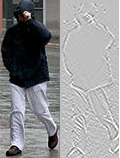
\includegraphics[width=0.5\linewidth]{figures/Pedestrian_gradient.jpg}
    \caption{An image of a pedestrian and gradient calculated by \acrshort{hog}.}
    \label{fig:pedestrian_gradient}
\end{figure}

Before the rise of deep learning, early computer vision research predominantly relied on manually engineered features. One of the influential approaches was the \acrfull{hog} introduced by \textcite{dalal_histogram_of_gradients}. \textcite{dalal_histogram_of_gradients} designed this method to detect humans in static images by partitioning an image into small regions, computing gradient directions within each patch, and ultimately assembling these measurements into a descriptive feature vector. \autoref{fig:pedestrian_gradient} visualizes the gradient vectors. Similarly, action recognition in videos was addressed through the Histogram of Flow\cite{dalal_histogram_of_flow}. This technique extends the \acrshort{hog} concept. The histogram of Flow calculates gradient descriptors at each frame.  It captures motion information through the analysis of optical flows, and then combines these per-frame descriptors into a representation that encapsulates temporal dynamics. \unsure{The HOG image is from Wikipedia, but they do not provide any source.}

Despite these approaches' innovation in early computer vision, their limitations soon became apparent. The reliance on accurate handcrafted features often led to challenges in scaling to complex scenarios and achieving generalization. Deep learning, with the ability to learn data-driven representations, has mainly outpaced these manual methods.

\subsection{Skeleton and Posture Estimation}
\label{ssec:skeleton_posture_estimation}

Skeleton and posture estimation techniques recover 2D or 3D joint coordinates from video frames to model player kinematics and pose dynamics \cite{elaoud_skeleton-based_2020, wang_skeleton_two-stream_2023, reilly__skeleton_just_pi_2023}. Common pipelines include:
\begin{itemize}
    \item Top-down methods: detect each player via bounding boxes, then apply a single-person pose estimator.
    \item Bottom-up methods: predict all joint candidates first and group them into skeletons.
    \item Graph-based models: use spatial-temporal graph convolutional networks (ST-GCN) to capture joint correlations over time\cite{yan_spatial_temporal_graph_convolutional_2018}.
\end{itemize}
These approaches extract features such as joint angles, stride length, and posture transitions for performance analysis and injury risk assessment. In football scenarios, however, they face:
\begin{itemize}
    \item Severe occlusions and player overlaps in crowded penalty areas.
    \item Varying camera angles, resolutions, and lens distortions.
    \item Fast motions causing motion blur and tracking drift\cite{survey_of_survey}.
\end{itemize} 


\section{Notation}
\label{sec:notation}
Let
\begin{itemize}
  \item $V=\{x_t\}_{t=1}^T$ be an input video of $T$ frames,
  \item $\mathcal{C}=\{1,\dots,12\}$ the set of action classes,
  \item $\mathcal{Y}=\{(t_i,c_i)\}_{i=1}^N$ the ground-truth annotations (timestamp $t_i$, class $c_i$),
  \item $\hat{\mathcal{Y}}=\{(\hat t_j,\hat c_j,\hat s_j)\}_{j=1}^M$ the model's predicted timestamps, classes, and confidence scores.
\end{itemize}
We consider a prediction $(\hat t_j,\hat c_j)$ correct if $\hat c_j=c_i$ and $|\hat t_j - t_i|\le\Delta$, where $\Delta$ is a fixed tolerance window (e.g.\ 1 s). Performance is measured by \acrfull{map} over all classes under the chosen $\Delta$.

\section{Temporal Modeling Techniques}\unsure{Should I remove this section}
\label{sec:temporal_models}

Temporal modeling techniques aim to capture motion and long-range dependencies across video frames. Common approaches include: \unsure{is this redundant}

\paragraph{\acrfull{rnn}}  
LSTM and GRU cells process a sequence of frame features \(x_t\in\mathbb{R}^d\) by carrying a hidden state \(h_t\):
\[
h_t = \mathrm{LSTM}(x_t,\,h_{t-1}), 
\qquad
\hat y_t = \mathrm{softmax}(W_o\,h_t + b_o).
\]
Gating mechanisms alleviate vanishing gradients but incur computation overhead.

\paragraph{Temporal Convolutional Networks (TCNs)}  
Dilated 1D convolutions aggregate information over multiple time steps in parallel:
\[
y_t = \sum_{k=0}^{K-1} w_k\,x_{t - d\,k} + b,
\]
where \(d\) is the dilation factor and \(K\) the kernel size. TCNs achieve large receptive fields with fewer layers.

\paragraph{Self-Attention Models}  
Transformers treat each frame's embedding as a token and apply multi-head attention:
\[
\mathrm{Attn}(Q,K,V) = \mathrm{softmax}\bigl(QK^\top/\sqrt{D}\bigr)\,V.
\]
They capture global context at a quadratic cost in sequence length.

\subsubsection{Temporal Segment Networks (TSN)}  
TSN splits a video into \(S\) segments, randomly samples one snippet per segment, extracts per-snippet features via a 2D \acrshort{cnn}, and fuses them with a consensus function (e.g., \ average pooling):
\[
F = \frac{1}{S}\sum_{s=1}^{S}f\bigl(\mathrm{CNN}(x_s)\bigr).
\]
By sparse sampling over long videos, TSN strikes a balance between efficiency and temporal coverage\cite{wang_tsn_2017}.

\section{Evaluation Metrics and Protocols}
\label{sec:evaluation}

\subsection{Spotting-Level Metrics}
\subsubsection{Mean Average Precision (mAP)}
We treat each predicted timestamp $\hat t_j$ and its corresponding class $\hat c_j$ as a detection. A true positive occurs if there exists a ground-truth event $(t_i,c_i)$ such that $\hat c_j = c_i$ and $|\hat t_j - t_i|\le\Delta$, where $\Delta$ is a fixed tolerance window (e.g.\ 1\,s). All unmatched predictions are false positives, and missed ground-truth events are false negatives. We compute precision-recall curves per class and report.
\[
\mathrm{AP}_c = \int_{0}^{1} p_c(r)\,\mathrm{d}r,\quad
\mathrm{mAP} = \frac{1}{|\mathcal{C}|}\sum_{c\in\mathcal{C}}\mathrm{AP}_c.
\]


% \subsection{Localization-Level Metrics}
% \subsubsection{\acrfull{iou}}
% For methods that predict temporal segments $[s_j,e_j]$, we measure overlap with ground-truth intervals $[t_i-\tfrac{\tau_i}{2},\,t_i+\tfrac{\tau_i}{2}]$ via
% \[
% \mathrm{IoU}([s_j,e_j],\,[g_s,g_e]) 
% = \frac{|[s_j,e_j]\cap [g_s,g_e]|}{|[s_j,e_j]\cup [g_s,g_e]|}.
% \]
% A segment is correct if $\mathrm{IoU}\!\ge\theta$ and $\hat c_j=c_i$.

% \subsubsection{mAP @ IoU Thresholds}
% \acrshort{map} is computed as above, replacing the tolerance criterion $|\hat t_j - t_i|\le\Delta$ with $\mathrm{IoU}\ge\theta$ for $\theta\in\{0.3,0.5,0.7\}$. This calculation compares single-timestamp spotting to full localization performance.


\subsection{Metrics Correlation and Importance}

\begin{figure}
    \centering
    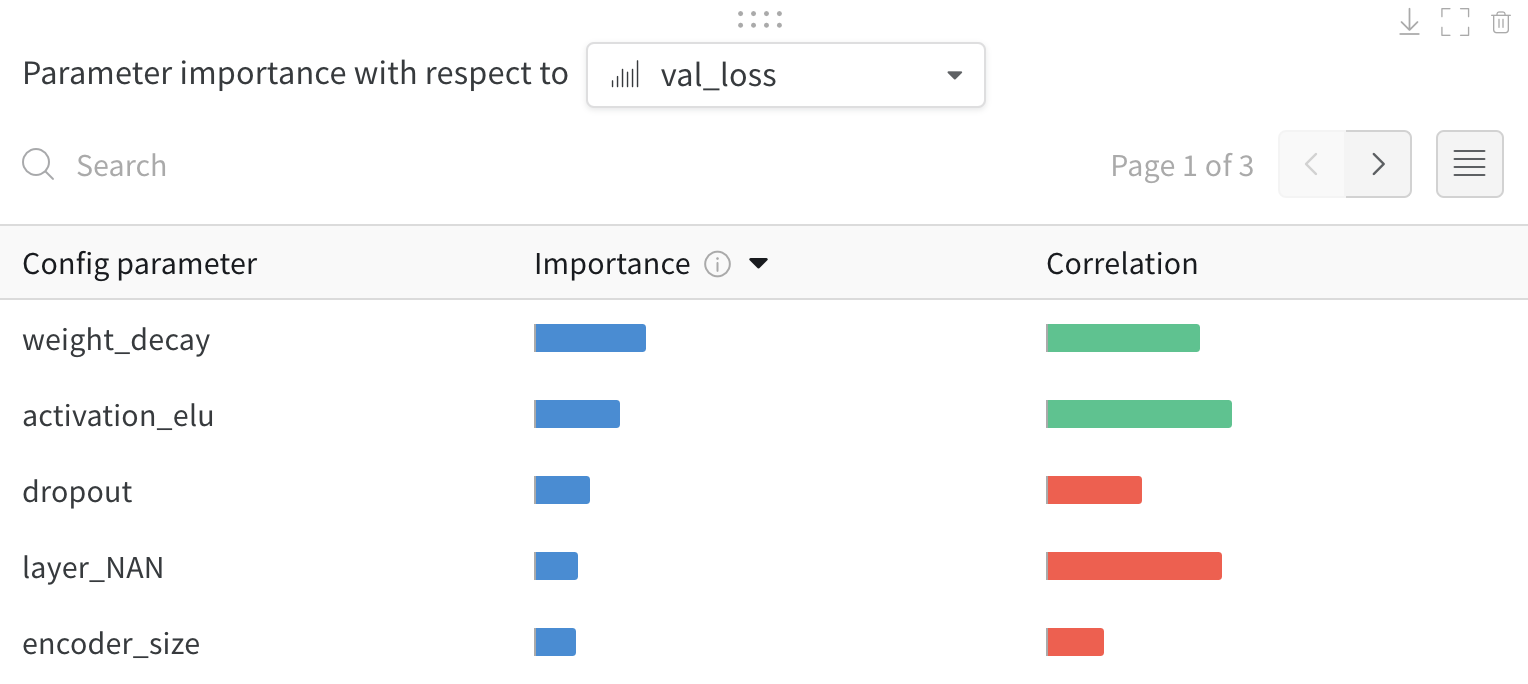
\includegraphics[width=0.5\linewidth]{figures/image.png}
    \caption{Example from \acrshort{wandb}\cite{wandb_parameter_importance} which shows the importance and correlation metric of a random project. The values indicate that correlation is not highly correlated with importance.}
    \label{fig:importance_v_correlation}
\end{figure}

\subsubsection{Correlation}

Correlation measures the linear relationship between parameters and a selected metric. In the case of hyperparameter searches, the linear relationship between validation loss and hyperparameter value is considered. A high correlation implies that an increase or decrease in the hyperparameter value leads to a similar change in the metric. However, correlation alone does not capture second-order interactions or non-linear dependencies.

\subsection{Importance}

To address these limitations, \acrfull{wandb} proposes an importance metric. The metric is derived using a random forest model trained with the hyperparameters as inputs. The target output is a performance metric. The feature importance values from this model provide deeper insights into which hyperparameters have a significant impact on the results. Unlike linear models, tree-based approaches are more robust to categorical data and non-normalized values\cite{wandb_parameter_importance}. As illustrated in \cref{fig:importance_v_correlation}, the importance metric can yield different insights compared to correlation-based methods and expose hidden relations.

\section{Related Work in Football Event Spotting}
\label{sec:fw_work}

\subsubsection{COMEDIAN}
COMEDIAN \cite{denize_comedian_2024} combines self-supervised learning and knowledge distillation to initialize a transformer for action-spotting on the SoccerNet-V2 dataset \cite{deliege_soccernet-v2_dataset_2021}. The contributions from Denize et al. include a three-step training pipeline and \acrlong{sota} performance. The first step is to use self-supervised pretraining on a spatial transformer. The second step is to initialize a temporal transformer using knowledge distillation to enrich the spatial transformer's output. The final step involves training on the relevant action spotting task, specifically SoccerNet-V2 \cite{deliege_soccernet-v2_dataset_2021}.

\subsubsection{\acrfull{tdeed}}
\acrlong{tdeed} \cite{xarles_t-deed_2024} won the action spotting category of SoccerNet 2024 \cite{cioppa_soccernet_2024}. The temporal part refers to looking at different lengths of time in the video. Discriminability ensures that each frame of the video is distinct. An encoder-decoder refers to the process of compressing and expanding video information. The model utilizes \acrfull{sgp} to enhance its discriminability between tokens. Enhanced discriminability is useful because sports actions can appear similar. 

\subsubsection{Group Activity Recognition}

In 2021, \textcite{gerats_individual_same_task_2021} utilized a single static panorama camera for action-spotting and activity recognition. The authors use player snippets as model input. Inflated 3D \acrshort{cnn} extracts spatio-temporal features from the snippets. A graph attention network analyzes the relationship between players and their activities and actions.

\section{Related Works in Action Localization}
\label{sec:related_works_all}

% \subsection{InternVideo 2}
\textcite{wang_internvideo2_2024} uses a 6B parameter video encoder in their InternVideo. It is a video foundation model, and the features extracted from the model are frequently used, e.g., in RDFA-S6.

% \subsubsection{RDFA-S6}
\textcite{lee_enhancing_mamba_s6_2024} enhances \acrshort{s6} into RDFA-S6 and specializes it towards the \acrshort{tal} domain. 

% \subsubsection{AdaTad}
\textcite{liu_adatad_2024} proposes the first end-to-end model which beats the feature based models on THUMOS14. The model builds on the Transformer architecture, and the authors emphasize the importance of scaling up a model to include more parameters. 

% \subsubsection{ActionFormer}
\textcite{zhang_actionformer_2022} utilized ActionFormer, which employed self-attention video transformers in 2022, to achieve a quantum leap in terms of \acrshort{tal} performance on THUMOS14. 

% \subsubsection{\acrfull{i3d} for Action Localization}
\textcite{host_handball_2023} uses \acrlong{i3d}s to detect actions in handball videos. 

\textcite{chen_children_2023} propose a combination of \acrfull{vlad} and \acrfull{dbn} to perform action recognition on football games with children. 

\textcite{wang_skeleton_two-stream_2023} combines a \acrfull{gcn} with transformers to understand human actions on a skeleton version of the Kinetics dataset.  \unsure{vlad and dbn not talked about earlier}

% \textcite{radhakrishnan_bi_lstm_2023} 
\textcite{giveki_human_2024} designs a novel \acrshort{gru} which focuses on spatial features, optical flow, and temporal dependencies to spot human actions. 
 

\unsure{To move all related work to the end or keep them together with their section}

% \todo{General feedback

% Prune repetitive definitions (RNN gating details, basic backpropagation) unless directly relevant.

% Use a neutral academic style: replace "this thesis" with "the present work" or "the proposed method."

% Check figure placement: Each significant concept benefits from a schematic (e.g., pipeline, masking schedule, SSM recurrence).

% Spell-check and unify acronym expansions on first use; remove stray unsure{} and todo{} comments}


\improvement{write about correlation?}

\todo{I could categorize all the articles in my Zotero to increase the length of the bibliography}